\documentclass[11pt]{article}
\usepackage[utf8]{inputenc}
\usepackage{graphicx} 
\usepackage[a4paper,top=2.54cm,bottom=2.54cm,left=2.54cm,right=2.54cm,marginparwidth=1.75cm]{geometry}
\usepackage{listings} %for code snipetts
\usepackage{xcolor}

\lstset{
    language=Python, 
    basicstyle=\ttfamily\footnotesize,     
    keywordstyle=\color{blue},        
    stringstyle=\color{teal},       
    commentstyle=\color{olive},      
    frame=single,                     
    rulecolor=\color{black},          
    breaklines=true,                
    showstringspaces=false          
}
\begin{document}


\begin{titlepage}
    \centering
    \vspace*{1cm} 
    \Huge
    \textbf{MNIST and CIFAR10 Neural Networks}
    \vspace{0.5cm} 
    \LARGE
    \\GRA-4152
    \vspace{1.5cm}
    \vfill 
    \Large
    BI Norwegian Business School\\
    \today 
\end{titlepage}


\section{NeuralNetwork: classes and subclasses}
\subsection{Inheritance diagram}
NeuralNetwork is the superclass of our project. This class is inherited by two subclasess: ConvNN and FullyConNN. The following image shows the inheritance diagram of our classes.
\begin{center}
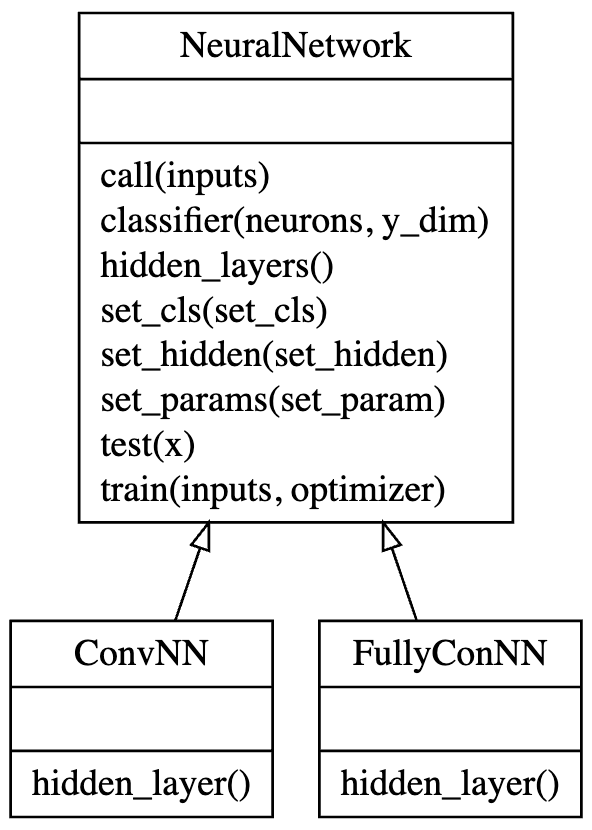
\includegraphics[width=0.4\textwidth]{NeuralNetwork.png}
\end{center}
The ConvNN and FullyConNN subclasses differ in the hidden\_layer method. This method creates the hidden layers for the different neural networks. The only inheritance that is not visible in the chart is that the NeuralNetwork superclass inherits from the tf.keras.Model class.\\ The public interface is different for the two subclasses. While for the ConvNN class, the user can define the input shape, neurons, filters, kernel size, and strides parameters, for the FullyConNN class the possible inputs are only input shape and neurons. Moreover, with creating an instance for any of these classes the constructor invokes all necessary methods thus the neural network is ready to be trained. In addition, the \_\_repr\_\_ method can be used to print information about the class.
\subsection{Methods used in these classes}
\begin{itemize}
\item \textbf{\_\_init\_\_():} the constructor of the superclass inherits the constructor from the keras Model class In addition, the constructor creates hidden, cls, params and neurons instance variables. Neurons instance variable is created in the superclass because we need the parameter both for the classifier and hidden\_layer method. The last method is only implemented in the subclass. This method receives as parameter the number of neurons for each layer in the hidden layers and the classifier.
\item \textbf{\_\_repr\_\_():} this method prints information about the class. This is an abstract method, implemented later in the subclass.
\item \textbf{hidden\_layers():} this method returns the hidden layers for a neural network. This is an abstract method, implemented later in the subclass.
\item \textbf{call():} this method returns the loss function based on the hidden and cls and the input values. Receives as parameters the inputs (x,y) a tuple where x is the input data and y is the result and returns the hidden layer object.
\item \textbf{classifier():} this method defines the classifier layer in the neural network. This layer is the same for both subclasses. Receives as parameters the number of classes in the classification task and returns the classifier layer object.
\item \textbf{train():} the train helps to train the model with the training data. Receives as parameters:
\begin{itemize}
            \item \textbf{inputs:} a tuple (x\_tr, y\_tr) wheres x is the training dataset and y is the training dataset in order to train the model.
            \item \textbf{optimizer:} optimizer algorithm to improve the weights in the neural networks. The default is Adam.
\end{itemize}
After the training, returns the loss function of the neural network.
\item \textbf{test():} The test method returns the estimated class and the probability for each class based on the trained model and the test set input values.
\item \textbf{set\_hidden():} this is an auxiliar method that sets the hidden instance variable to a new object.
\item \textbf{set\_params():} this is an auxiliar method that sets the trainable parameters to a new object.
\item \textbf{set\_cls():} this is an auxiliar method that sets the parameters of the classifier layer.
\end{itemize}

\subsection{Inheritance, overriding and polymorphism}
\emph{Inheritance:} we used inheritance first when the NeuralNetwork class inherited from the keras Model class. Then the subclasses, ConvNN and FullyConNN inherited the implemented methods from NeuralNetwork superclass. For instance, the classifier method should be implemented in the same way for both subclasses, therefore it can be implemented in the superclass.
\\
\\
\emph{Overriding:}  is used for example in the case of the call method that is inherited from tf.keras.Model class. In the NeuralNetworks class we override the call method to give us the chosen loss function.
\\
\\
\emph{Polymorphism:}  is used for the hidden\_layer method. Both subclasses should have this method, but the implementation should be different for these classes. Therefore, first, we created an abstract method in the NeuralNetworks superclass, and this method is inherited by the subclasses. In the subclasses this not implemented method is overridden in a different way for the different classes. Finally, this hidden\_layer method is implemented for all subclasses but works in a different way.


\section{Dataloader: classes and subclasses}
\subsection{Inheritance diagram}
DataLoader is another superclass of our project. This class is not as important as important as NeuralNetwork but it plays a vital role by being responsible for loading the data correctly. DataLoader has two subclasses: MNIST and CIFAR10, these are used to load specific datasets. The following image shows the inheritance diagram of our classes.
\begin{center}
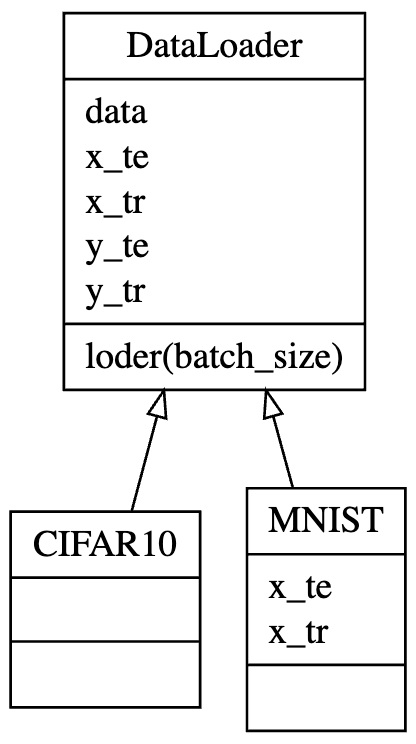
\includegraphics[width=0.4\textwidth]{dataloader.png}
\end{center}
Both CIFAR10 and MNIST extend the constructor method of DataLoader loading the keras datasets CIFAR10 and MNIST respectively. For the MNIST class specifically the methods x\_te and x\_tr are overriden in order to change the shape of the arrays that they return.

\subsection{Methods used in the class}
Both MNIST and CIFAR10 have two types of methods:
\begin{itemize}
\item \textbf{Accessor methods:}  there are 5 accessor methods in each class \emph{data, x\_te, x\_tr, y\_te} and \emph{y\_tr}
	\begin{itemize}
	\item \textbf{data:} returns a tuple with the training and test datasets
	\item \textbf{x\_te, x\_tr, y\_te} and \textbf{y\_tr:} return a specific part of data. This can be either a training or test dataset and can be for either the group of independent variables or for the dependent variable.
	\end{itemize}
\item \textbf{loder:} this is the main method of the class, receives as an input the number of batches to be train and returns an array of this size of tuples containing the independent variables and the dependent variable.
\end{itemize}

\subsection{Inheritance, overriding}
\emph{Inheritance:} is used in every method, but  for all the methods of CIFAR10 and for the methods  \emph{data, y\_te, y\_tr} and \emph{loder} not overriding is required and its final implementation is completely inherited from the DataLoader super class.
\\
\\
\emph{Overriding:}  is used in \_\_init\_\_() method to load either the MNIST or CIFAR10 dataset. Additionally in MNIST is used in \emph {x\_tr} and \emph{x\_te} to the extend the functionality of these methods. Firstly the super method is inherited and then its output is reshaped to a more suitable form to be trained later by the neural networks.
\section{Training and testing}
To train and test the model a specific file was created \emph{train.py}. This file takes advantage of the argparse class in python in order to receive parameters and to test the neural networks.
The argparse has two components
\begin{itemize}
\item \textbf{doc:} this argument needs to be specified in order to get access to the documentation of the classes. To get the documentation, the class name is needed. Additionally, the methods argument can be specified to get the documentation of each method in the class:
\begin{lstlisting}
 python train.py --doc --class_name CIFAR10 --methods
\end{lstlisting}

\item \textbf{test:} this argument is used to test the neural networks. The batch size, the number of epochs to be trained, the dataset, the type of neural network and the number of neurons of the model can all be modified to test the program.
\begin{lstlisting}
 python train.py --test --dset cifar10 --nn_type ConvNN --epochs 10
 python train.py --test --dset mnist --nn_type FullyConNN --epochs 10
\end{lstlisting}
\end{itemize}


\end{document}

